\documentclass[border=10pt,varwidth=\maxdimen]{standalone}

\usepackage{verbatim}
\usepackage{tikz}
\usetikzlibrary{calc, shapes, backgrounds,graphs,positioning,fit}
\usetikzlibrary{bayesnet}
\usetikzlibrary{arrows}

\usepackage{amsmath, amssymb}
\usepackage{graphicx}

\begin{document}
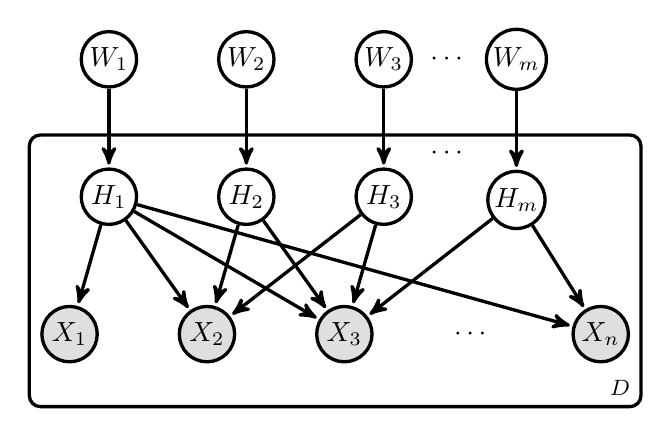
\begin{tikzpicture}[->,>=stealth',shorten >=1pt,auto,node distance=3cm, very thick]
    % Define nodes
    \node[latent] (W1) {$W_1$};
    \node[latent, right=of W1] (W2) {$W_2$};
    \node[latent, right=of W2] (W3) {$W_3$};
    \node[const, right=of W3, xshift=-0.8cm] (W4) {$\cdots$};
    \node[latent, right=of W4, xshift=-0.8cm] (W5) {$W_m$};

    \node[latent, below=of W1] (H1) {$H_1$};
    \node[latent, below=of W2] (H2) {$H_2$};
    \node[latent, below=of W3] (H3) {$H_3$};
    \node[const, below=of W4] (H4) {$\cdots$};
    \node[latent, below=of W5] (H5) {$H_m$};

    \node[obs, below=of H1, xshift=-0.5cm] (X1) {$X_1$};
    \node[obs, right=of X1] (X2) {$X_2$};
    \node[obs, right=of X2] (X3) {$X_3$};
    \node[const, right=of X3] (X4) {$\cdots$};
    \node[obs, right=of X4] (X5) {$X_n$};

    \draw (W1) -- (H1);
    \draw (W2) -- (H2);
    \draw (W3) -- (H3);
    \draw (W5) -- (H5);

    \draw (H1) -- (X1);
    \draw (H1) -- (X2);
    \draw (H1) -- (X3);
    \draw (H1) -- (X5);

    \draw (H2) -- (X2);
    \draw (H2) -- (X3);

    \draw (H3) -- (X2);
    \draw (H3) -- (X3);

    \draw (H5) -- (X3);
    \draw (H5) -- (X5);

    \plate {} {(H1)(H2)(H3)(H4)(H5)(X1)(X2)(X3)(X4)(X5)} {$D$};

\end{tikzpicture}
\end{document}

